\chapter{Implementazione}
\section{Struttura del progetto}
La struttura del progetto, organizzato in package, è la seguente:
\begin{itemize}
    \item \textbf{Actions}: le azioni della simulazione.
    \item \textbf{GlobalActions}: le azioni globali della simulazione.
    \item \textbf{Layer}: il layer personalizzato della simulazione.
    \item \textbf{NodeProperty}: le proprietà dei nodi della simulazione.
\end{itemize}
\clearpage
\section{Layer}
\begin{figure}[ht]
    \centering
    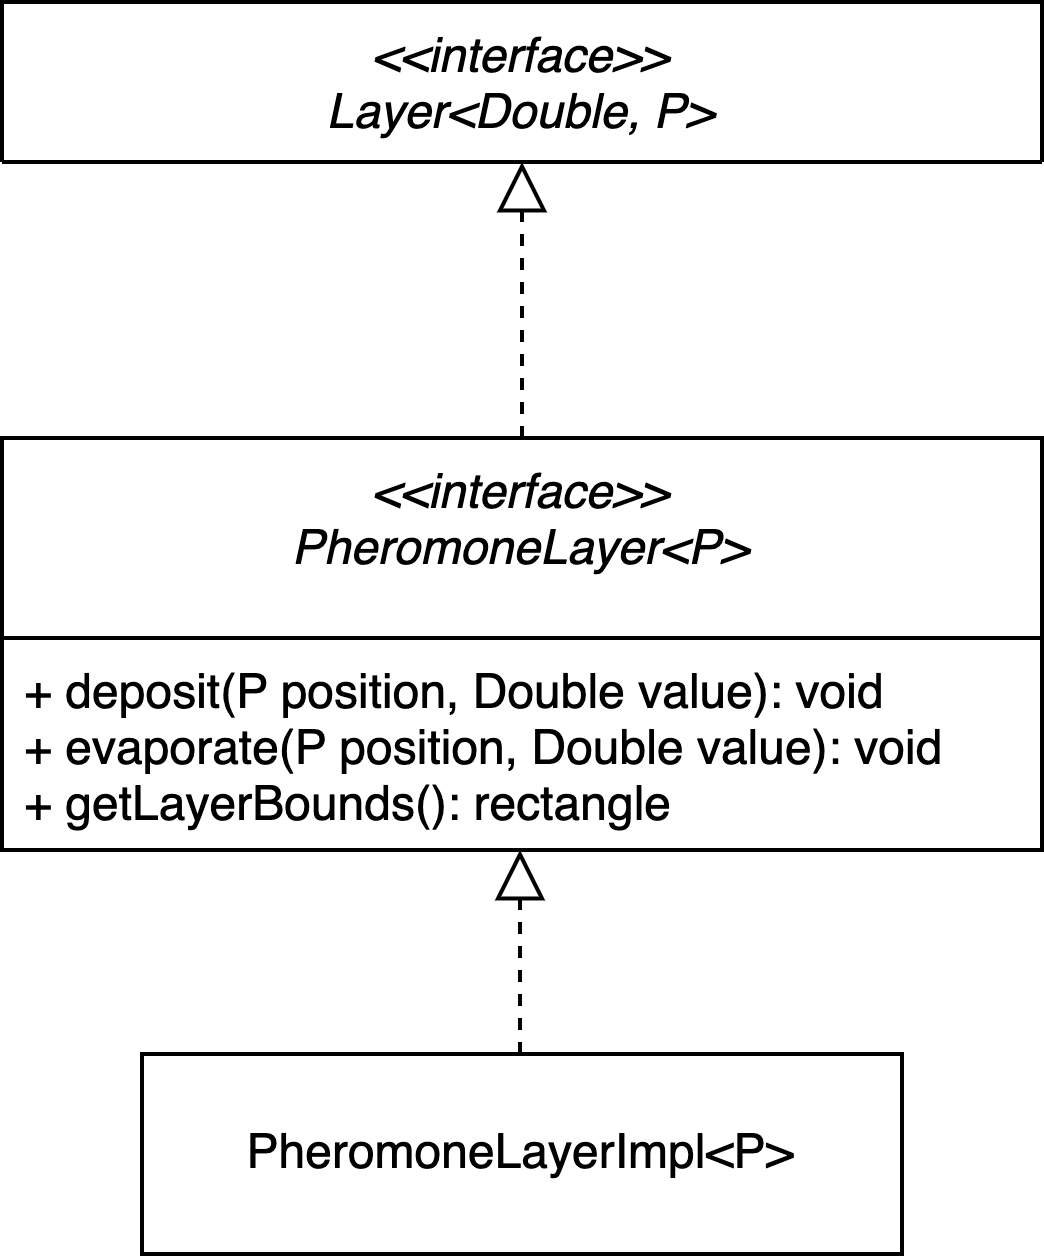
\includegraphics[width=.5\linewidth]{figures/pheromoneLayer.png}
    \caption{Struttura PheromoneLayer}\label{fig:phLayer}
\end{figure}
Il \texttt{PheromoneLayer<P extends Position2D<P>>}, layer personalizzato della simulazione, è stato implementato 
come una interfaccia che estende \texttt{Layer<T, P>}, dove \texttt{T} è il tipo di nodo e \texttt{P} è il tipo di posizione,
interfaccia propria di Alchemist. L'utilizzo del parametro \texttt{P} implica che il \texttt{PheromoneLayer} può essere utilizzato con qualsiasi tipo di posizione, ma
è stato pensato per sfruttare le posizioni \texttt{Position2D<P>} bidimensionali.
Per la sua creazione è necessario definire 5 misure:
\begin{itemize}
    \item \texttt{startX}: la coordinata x di partenza.
    \item \texttt{startY}: la coordinata y di partenza.
    \item \texttt{width}: la larghezza del layer.
    \item \texttt{height}: l'altezza del layer.
    \item \texttt{step}: la dimensione del passo, ovvero la lunghezza del lato di ogni \textit{patch}.
\end{itemize}
Lo \texttt{step} è un parametro fondamentale per la corretta implementazione della simulazione
in quanto Alchemist non possiede il concetto di area, necessaria per individuare una \textit{patch}.
Queste vengono rappresentate come ``aree'' puntiformi, e la loro dimensione (ovvero la distanza di un punto dall'altro) è appunto definita da questo parametro.
Nella simulazione, il nodo deposita il feromone in una qualsiasi posizione, discreta e non obbligatoriamente intera, all'interno dei limiti dello spazio, e il \texttt{PheromoneLayer} 
si occupa di convertire questa posizione in una appartenente ad una \textit{patch}. 
Esegue quindi un arrotondamento per eccesso o per difetto, in modo tale da ottenere la posizione della \textit{patch} più vicina.
\begin{figure}[ht]
    \centering
    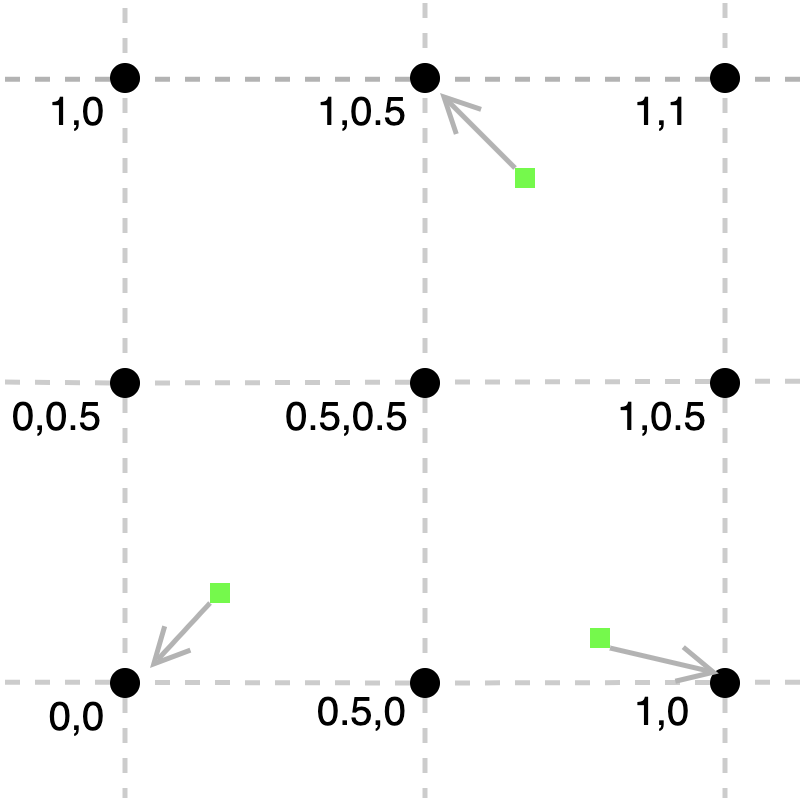
\includegraphics[width=.5\linewidth]{figures/patch-nodi.png}
    \caption{Rappresentazione grafica delle \textit{patches} puntiformi. Ogni punto rappresenta una patch,
    mentre i quadratini rappresentano i nodi e la freccia indica su che \textit{patch} il nodo depositerà il feromone. In questo esempio
    startX e startY hanno come valore 0, width e height 1 e step 0.5}\label{fig:patch-nodi}
\end{figure}
%devo parlare della Mappa e delle posizioni, di come vengono convertite magari aggiungendo delle foto.
\subsection{Struttura dati}
Un aspetto di fondamentale importanza riguarda la struttura dati utilizzata per la gestione del feromone.
Per ovviare alla mancanza del concetto di area, è stato utilizzato un \texttt{HashMap<P, Double>} che associa ad ogni posizione \texttt{P} un valore \texttt{Double} di feromone.
Questa mappa viene inizializzata nel costruttore della classe attraverso il metodo \texttt{setupEnviromnent()} che si occupa di popolare la mappa
con tutte le possibili posizioni delle \textit{patch} e di inizializzare il feromone a 0.
\lstinputlisting[language=Java,label={lst:phlayer}]{listings/phlayersetup.java}
\subsection{Metodi}
I metodi definiti nell'interfaccia e implementati nella classe sono:
\begin{itemize}
    \item \texttt{void evaporate(P position, Double value)}: metodo che permette di far evaporare il feromone. 
    Richiede in input la posizione e il valore del feromone.
    \item \texttt{void deposit(P position, Double value)}: metodo che permette di far diffondere il feromone.
     Richiede in input la posizione e il valore del feromone.
    \item \texttt{Rectangle getLayerBounds()}: metodo che restituisce un oggetto di tipo \texttt{Rectangle}.
\end{itemize}


